% Created by tikzDevice version 0.12.6 on 2023-12-15 16:10:39
% !TEX encoding = UTF-8 Unicode
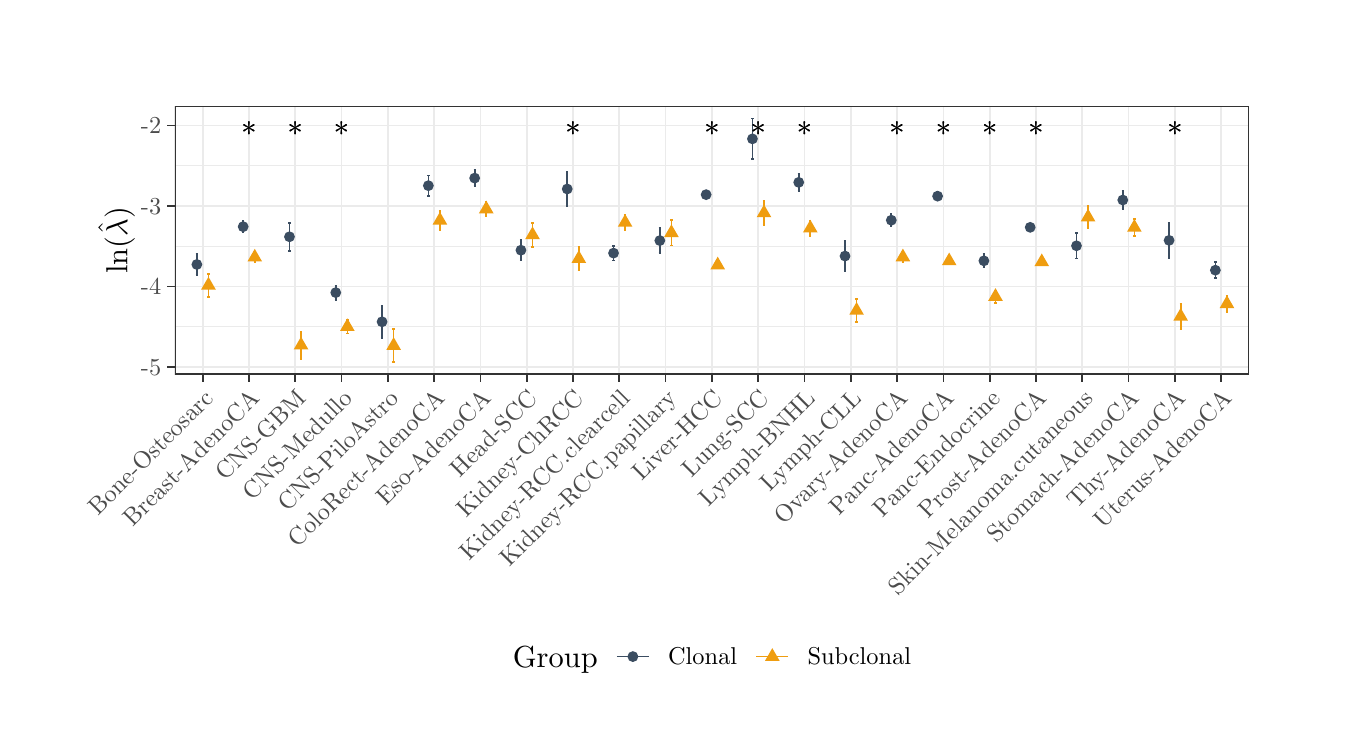
\begin{tikzpicture}[x=1pt,y=1pt]
\definecolor{fillColor}{RGB}{255,255,255}
\path[use as bounding box,fill=fillColor,fill opacity=0.00] (0,0) rectangle (469.75,252.94);
\begin{scope}
\path[clip] (  0.00,  0.00) rectangle (469.75,252.94);
\definecolor{drawColor}{RGB}{255,255,255}
\definecolor{fillColor}{RGB}{255,255,255}

\path[draw=drawColor,line width= 0.6pt,line join=round,line cap=round,fill=fillColor] (  0.00,  0.00) rectangle (469.76,252.95);
\end{scope}
\begin{scope}
\path[clip] ( 53.20,127.70) rectangle (441.30,224.49);
\definecolor{fillColor}{RGB}{255,255,255}

\path[fill=fillColor] ( 53.20,127.70) rectangle (441.30,224.49);
\definecolor{drawColor}{gray}{0.92}

\path[draw=drawColor,line width= 0.3pt,line join=round] ( 53.20,144.94) --
	(441.30,144.94);

\path[draw=drawColor,line width= 0.3pt,line join=round] ( 53.20,173.99) --
	(441.30,173.99);

\path[draw=drawColor,line width= 0.3pt,line join=round] ( 53.20,203.03) --
	(441.30,203.03);

\path[draw=drawColor,line width= 0.6pt,line join=round] ( 53.20,130.42) --
	(441.30,130.42);

\path[draw=drawColor,line width= 0.6pt,line join=round] ( 53.20,159.47) --
	(441.30,159.47);

\path[draw=drawColor,line width= 0.6pt,line join=round] ( 53.20,188.51) --
	(441.30,188.51);

\path[draw=drawColor,line width= 0.6pt,line join=round] ( 53.20,217.55) --
	(441.30,217.55);

\path[draw=drawColor,line width= 0.6pt,line join=round] ( 63.24,127.70) --
	( 63.24,224.49);

\path[draw=drawColor,line width= 0.6pt,line join=round] ( 79.96,127.70) --
	( 79.96,224.49);

\path[draw=drawColor,line width= 0.6pt,line join=round] ( 96.69,127.70) --
	( 96.69,224.49);

\path[draw=drawColor,line width= 0.6pt,line join=round] (113.42,127.70) --
	(113.42,224.49);

\path[draw=drawColor,line width= 0.6pt,line join=round] (130.15,127.70) --
	(130.15,224.49);

\path[draw=drawColor,line width= 0.6pt,line join=round] (146.88,127.70) --
	(146.88,224.49);

\path[draw=drawColor,line width= 0.6pt,line join=round] (163.61,127.70) --
	(163.61,224.49);

\path[draw=drawColor,line width= 0.6pt,line join=round] (180.34,127.70) --
	(180.34,224.49);

\path[draw=drawColor,line width= 0.6pt,line join=round] (197.06,127.70) --
	(197.06,224.49);

\path[draw=drawColor,line width= 0.6pt,line join=round] (213.79,127.70) --
	(213.79,224.49);

\path[draw=drawColor,line width= 0.6pt,line join=round] (230.52,127.70) --
	(230.52,224.49);

\path[draw=drawColor,line width= 0.6pt,line join=round] (247.25,127.70) --
	(247.25,224.49);

\path[draw=drawColor,line width= 0.6pt,line join=round] (263.98,127.70) --
	(263.98,224.49);

\path[draw=drawColor,line width= 0.6pt,line join=round] (280.71,127.70) --
	(280.71,224.49);

\path[draw=drawColor,line width= 0.6pt,line join=round] (297.44,127.70) --
	(297.44,224.49);

\path[draw=drawColor,line width= 0.6pt,line join=round] (314.16,127.70) --
	(314.16,224.49);

\path[draw=drawColor,line width= 0.6pt,line join=round] (330.89,127.70) --
	(330.89,224.49);

\path[draw=drawColor,line width= 0.6pt,line join=round] (347.62,127.70) --
	(347.62,224.49);

\path[draw=drawColor,line width= 0.6pt,line join=round] (364.35,127.70) --
	(364.35,224.49);

\path[draw=drawColor,line width= 0.6pt,line join=round] (381.08,127.70) --
	(381.08,224.49);

\path[draw=drawColor,line width= 0.6pt,line join=round] (397.81,127.70) --
	(397.81,224.49);

\path[draw=drawColor,line width= 0.6pt,line join=round] (414.54,127.70) --
	(414.54,224.49);

\path[draw=drawColor,line width= 0.6pt,line join=round] (431.27,127.70) --
	(431.27,224.49);
\definecolor{fillColor}{RGB}{59,77,97}

\path[fill=fillColor] ( 61.14,167.37) circle (  1.96);
\definecolor{fillColor}{RGB}{239,157,16}

\path[fill=fillColor] ( 65.33,162.90) --
	( 67.97,158.32) --
	( 62.68,158.32) --
	cycle;
\definecolor{fillColor}{RGB}{59,77,97}

\path[fill=fillColor] ( 77.87,181.03) circle (  1.96);
\definecolor{fillColor}{RGB}{239,157,16}

\path[fill=fillColor] ( 82.06,173.02) --
	( 84.70,168.45) --
	( 79.41,168.45) --
	cycle;
\definecolor{fillColor}{RGB}{59,77,97}

\path[fill=fillColor] ( 94.60,177.38) circle (  1.96);
\definecolor{fillColor}{RGB}{239,157,16}

\path[fill=fillColor] ( 98.78,141.25) --
	(101.43,136.67) --
	( 96.14,136.67) --
	cycle;
\definecolor{fillColor}{RGB}{59,77,97}

\path[fill=fillColor] (111.33,157.20) circle (  1.96);
\definecolor{fillColor}{RGB}{239,157,16}

\path[fill=fillColor] (115.51,147.91) --
	(118.16,143.34) --
	(112.87,143.34) --
	cycle;
\definecolor{fillColor}{RGB}{59,77,97}

\path[fill=fillColor] (128.06,146.66) circle (  1.96);
\definecolor{fillColor}{RGB}{239,157,16}

\path[fill=fillColor] (132.24,141.11) --
	(134.88,136.54) --
	(129.60,136.54) --
	cycle;
\definecolor{fillColor}{RGB}{59,77,97}

\path[fill=fillColor] (144.79,195.85) circle (  1.96);
\definecolor{fillColor}{RGB}{239,157,16}

\path[fill=fillColor] (148.97,186.36) --
	(151.61,181.79) --
	(146.33,181.79) --
	cycle;
\definecolor{fillColor}{RGB}{59,77,97}

\path[fill=fillColor] (161.52,198.58) circle (  1.96);
\definecolor{fillColor}{RGB}{239,157,16}

\path[fill=fillColor] (165.70,190.44) --
	(168.34,185.87) --
	(163.06,185.87) --
	cycle;
\definecolor{fillColor}{RGB}{59,77,97}

\path[fill=fillColor] (178.24,172.53) circle (  1.96);
\definecolor{fillColor}{RGB}{239,157,16}

\path[fill=fillColor] (182.43,181.10) --
	(185.07,176.53) --
	(179.78,176.53) --
	cycle;
\definecolor{fillColor}{RGB}{59,77,97}

\path[fill=fillColor] (194.97,194.65) circle (  1.96);
\definecolor{fillColor}{RGB}{239,157,16}

\path[fill=fillColor] (199.16,172.53) --
	(201.80,167.95) --
	(196.51,167.95) --
	cycle;
\definecolor{fillColor}{RGB}{59,77,97}

\path[fill=fillColor] (211.70,171.48) circle (  1.96);
\definecolor{fillColor}{RGB}{239,157,16}

\path[fill=fillColor] (215.88,185.59) --
	(218.53,181.01) --
	(213.24,181.01) --
	cycle;
\definecolor{fillColor}{RGB}{59,77,97}

\path[fill=fillColor] (228.43,176.00) circle (  1.96);
\definecolor{fillColor}{RGB}{239,157,16}

\path[fill=fillColor] (232.61,181.85) --
	(235.26,177.27) --
	(229.97,177.27) --
	cycle;
\definecolor{fillColor}{RGB}{59,77,97}

\path[fill=fillColor] (245.16,192.60) circle (  1.96);
\definecolor{fillColor}{RGB}{239,157,16}

\path[fill=fillColor] (249.34,170.19) --
	(251.98,165.62) --
	(246.70,165.62) --
	cycle;
\definecolor{fillColor}{RGB}{59,77,97}

\path[fill=fillColor] (261.89,212.76) circle (  1.96);
\definecolor{fillColor}{RGB}{239,157,16}

\path[fill=fillColor] (266.07,189.03) --
	(268.71,184.46) --
	(263.43,184.46) --
	cycle;
\definecolor{fillColor}{RGB}{59,77,97}

\path[fill=fillColor] (278.62,197.04) circle (  1.96);
\definecolor{fillColor}{RGB}{239,157,16}

\path[fill=fillColor] (282.80,183.53) --
	(285.44,178.96) --
	(280.16,178.96) --
	cycle;
\definecolor{fillColor}{RGB}{59,77,97}

\path[fill=fillColor] (295.35,170.41) circle (  1.96);
\definecolor{fillColor}{RGB}{239,157,16}

\path[fill=fillColor] (299.53,153.79) --
	(302.17,149.21) --
	(296.88,149.21) --
	cycle;
\definecolor{fillColor}{RGB}{59,77,97}

\path[fill=fillColor] (312.07,183.36) circle (  1.96);
\definecolor{fillColor}{RGB}{239,157,16}

\path[fill=fillColor] (316.26,173.10) --
	(318.90,168.53) --
	(313.61,168.53) --
	cycle;
\definecolor{fillColor}{RGB}{59,77,97}

\path[fill=fillColor] (328.80,192.05) circle (  1.96);
\definecolor{fillColor}{RGB}{239,157,16}

\path[fill=fillColor] (332.98,171.68) --
	(335.63,167.10) --
	(330.34,167.10) --
	cycle;
\definecolor{fillColor}{RGB}{59,77,97}

\path[fill=fillColor] (345.53,168.69) circle (  1.96);
\definecolor{fillColor}{RGB}{239,157,16}

\path[fill=fillColor] (349.71,158.81) --
	(352.36,154.24) --
	(347.07,154.24) --
	cycle;
\definecolor{fillColor}{RGB}{59,77,97}

\path[fill=fillColor] (362.26,180.79) circle (  1.96);
\definecolor{fillColor}{RGB}{239,157,16}

\path[fill=fillColor] (366.44,171.34) --
	(369.08,166.77) --
	(363.80,166.77) --
	cycle;
\definecolor{fillColor}{RGB}{59,77,97}

\path[fill=fillColor] (378.99,174.12) circle (  1.96);
\definecolor{fillColor}{RGB}{239,157,16}

\path[fill=fillColor] (383.17,187.51) --
	(385.81,182.93) --
	(380.53,182.93) --
	cycle;
\definecolor{fillColor}{RGB}{59,77,97}

\path[fill=fillColor] (395.72,190.66) circle (  1.96);
\definecolor{fillColor}{RGB}{239,157,16}

\path[fill=fillColor] (399.90,183.79) --
	(402.54,179.21) --
	(397.26,179.21) --
	cycle;
\definecolor{fillColor}{RGB}{59,77,97}

\path[fill=fillColor] (412.45,176.08) circle (  1.96);
\definecolor{fillColor}{RGB}{239,157,16}

\path[fill=fillColor] (416.63,151.67) --
	(419.27,147.09) --
	(413.99,147.09) --
	cycle;
\definecolor{fillColor}{RGB}{59,77,97}

\path[fill=fillColor] (429.17,165.30) circle (  1.96);
\definecolor{fillColor}{RGB}{239,157,16}

\path[fill=fillColor] (433.36,156.20) --
	(436.00,151.62) --
	(430.71,151.62) --
	cycle;
\definecolor{drawColor}{RGB}{59,77,97}

\path[draw=drawColor,line width= 0.6pt,line join=round] ( 60.73,171.25) --
	( 61.56,171.25);

\path[draw=drawColor,line width= 0.6pt,line join=round] ( 61.14,171.25) --
	( 61.14,163.50);

\path[draw=drawColor,line width= 0.6pt,line join=round] ( 60.73,163.50) --
	( 61.56,163.50);
\definecolor{drawColor}{RGB}{239,157,16}

\path[draw=drawColor,line width= 0.6pt,line join=round] ( 64.91,164.02) --
	( 65.75,164.02);

\path[draw=drawColor,line width= 0.6pt,line join=round] ( 65.33,164.02) --
	( 65.33,155.67);

\path[draw=drawColor,line width= 0.6pt,line join=round] ( 64.91,155.67) --
	( 65.75,155.67);
\definecolor{drawColor}{RGB}{59,77,97}

\path[draw=drawColor,line width= 0.6pt,line join=round] ( 77.46,182.98) --
	( 78.29,182.98);

\path[draw=drawColor,line width= 0.6pt,line join=round] ( 77.87,182.98) --
	( 77.87,179.08);

\path[draw=drawColor,line width= 0.6pt,line join=round] ( 77.46,179.08) --
	( 78.29,179.08);
\definecolor{drawColor}{RGB}{239,157,16}

\path[draw=drawColor,line width= 0.6pt,line join=round] ( 81.64,171.78) --
	( 82.47,171.78);

\path[draw=drawColor,line width= 0.6pt,line join=round] ( 82.06,171.78) --
	( 82.06,168.17);

\path[draw=drawColor,line width= 0.6pt,line join=round] ( 81.64,168.17) --
	( 82.47,168.17);
\definecolor{drawColor}{RGB}{59,77,97}

\path[draw=drawColor,line width= 0.6pt,line join=round] ( 94.18,182.45) --
	( 95.02,182.45);

\path[draw=drawColor,line width= 0.6pt,line join=round] ( 94.60,182.45) --
	( 94.60,172.30);

\path[draw=drawColor,line width= 0.6pt,line join=round] ( 94.18,172.30) --
	( 95.02,172.30);
\definecolor{drawColor}{RGB}{239,157,16}

\path[draw=drawColor,line width= 0.6pt,line join=round] ( 98.37,143.15) --
	( 99.20,143.15);

\path[draw=drawColor,line width= 0.6pt,line join=round] ( 98.78,143.15) --
	( 98.78,133.24);

\path[draw=drawColor,line width= 0.6pt,line join=round] ( 98.37,133.24) --
	( 99.20,133.24);
\definecolor{drawColor}{RGB}{59,77,97}

\path[draw=drawColor,line width= 0.6pt,line join=round] (110.91,159.77) --
	(111.75,159.77);

\path[draw=drawColor,line width= 0.6pt,line join=round] (111.33,159.77) --
	(111.33,154.63);

\path[draw=drawColor,line width= 0.6pt,line join=round] (110.91,154.63) --
	(111.75,154.63);
\definecolor{drawColor}{RGB}{239,157,16}

\path[draw=drawColor,line width= 0.6pt,line join=round] (115.09,147.30) --
	(115.93,147.30);

\path[draw=drawColor,line width= 0.6pt,line join=round] (115.51,147.30) --
	(115.51,142.42);

\path[draw=drawColor,line width= 0.6pt,line join=round] (115.09,142.42) --
	(115.93,142.42);
\definecolor{drawColor}{RGB}{59,77,97}

\path[draw=drawColor,line width= 0.6pt,line join=round] (127.64,152.50) --
	(128.48,152.50);

\path[draw=drawColor,line width= 0.6pt,line join=round] (128.06,152.50) --
	(128.06,140.81);

\path[draw=drawColor,line width= 0.6pt,line join=round] (127.64,140.81) --
	(128.48,140.81);
\definecolor{drawColor}{RGB}{239,157,16}

\path[draw=drawColor,line width= 0.6pt,line join=round] (131.82,144.02) --
	(132.66,144.02);

\path[draw=drawColor,line width= 0.6pt,line join=round] (132.24,144.02) --
	(132.24,132.10);

\path[draw=drawColor,line width= 0.6pt,line join=round] (131.82,132.10) --
	(132.66,132.10);
\definecolor{drawColor}{RGB}{59,77,97}

\path[draw=drawColor,line width= 0.6pt,line join=round] (144.37,199.55) --
	(145.21,199.55);

\path[draw=drawColor,line width= 0.6pt,line join=round] (144.79,199.55) --
	(144.79,192.15);

\path[draw=drawColor,line width= 0.6pt,line join=round] (144.37,192.15) --
	(145.21,192.15);
\definecolor{drawColor}{RGB}{239,157,16}

\path[draw=drawColor,line width= 0.6pt,line join=round] (148.55,186.71) --
	(149.39,186.71);

\path[draw=drawColor,line width= 0.6pt,line join=round] (148.97,186.71) --
	(148.97,179.91);

\path[draw=drawColor,line width= 0.6pt,line join=round] (148.55,179.91) --
	(149.39,179.91);
\definecolor{drawColor}{RGB}{59,77,97}

\path[draw=drawColor,line width= 0.6pt,line join=round] (161.10,201.46) --
	(161.93,201.46);

\path[draw=drawColor,line width= 0.6pt,line join=round] (161.52,201.46) --
	(161.52,195.69);

\path[draw=drawColor,line width= 0.6pt,line join=round] (161.10,195.69) --
	(161.93,195.69);
\definecolor{drawColor}{RGB}{239,157,16}

\path[draw=drawColor,line width= 0.6pt,line join=round] (165.28,189.90) --
	(166.12,189.90);

\path[draw=drawColor,line width= 0.6pt,line join=round] (165.70,189.90) --
	(165.70,184.88);

\path[draw=drawColor,line width= 0.6pt,line join=round] (165.28,184.88) --
	(166.12,184.88);
\definecolor{drawColor}{RGB}{59,77,97}

\path[draw=drawColor,line width= 0.6pt,line join=round] (177.83,176.22) --
	(178.66,176.22);

\path[draw=drawColor,line width= 0.6pt,line join=round] (178.24,176.22) --
	(178.24,168.84);

\path[draw=drawColor,line width= 0.6pt,line join=round] (177.83,168.84) --
	(178.66,168.84);
\definecolor{drawColor}{RGB}{239,157,16}

\path[draw=drawColor,line width= 0.6pt,line join=round] (182.01,182.42) --
	(182.85,182.42);

\path[draw=drawColor,line width= 0.6pt,line join=round] (182.43,182.42) --
	(182.43,173.69);

\path[draw=drawColor,line width= 0.6pt,line join=round] (182.01,173.69) --
	(182.85,173.69);
\definecolor{drawColor}{RGB}{59,77,97}

\path[draw=drawColor,line width= 0.6pt,line join=round] (194.56,200.76) --
	(195.39,200.76);

\path[draw=drawColor,line width= 0.6pt,line join=round] (194.97,200.76) --
	(194.97,188.54);

\path[draw=drawColor,line width= 0.6pt,line join=round] (194.56,188.54) --
	(195.39,188.54);
\definecolor{drawColor}{RGB}{239,157,16}

\path[draw=drawColor,line width= 0.6pt,line join=round] (198.74,173.82) --
	(199.57,173.82);

\path[draw=drawColor,line width= 0.6pt,line join=round] (199.16,173.82) --
	(199.16,165.14);

\path[draw=drawColor,line width= 0.6pt,line join=round] (198.74,165.14) --
	(199.57,165.14);
\definecolor{drawColor}{RGB}{59,77,97}

\path[draw=drawColor,line width= 0.6pt,line join=round] (211.28,174.10) --
	(212.12,174.10);

\path[draw=drawColor,line width= 0.6pt,line join=round] (211.70,174.10) --
	(211.70,168.86);

\path[draw=drawColor,line width= 0.6pt,line join=round] (211.28,168.86) --
	(212.12,168.86);
\definecolor{drawColor}{RGB}{239,157,16}

\path[draw=drawColor,line width= 0.6pt,line join=round] (215.47,185.23) --
	(216.30,185.23);

\path[draw=drawColor,line width= 0.6pt,line join=round] (215.88,185.23) --
	(215.88,179.85);

\path[draw=drawColor,line width= 0.6pt,line join=round] (215.47,179.85) --
	(216.30,179.85);
\definecolor{drawColor}{RGB}{59,77,97}

\path[draw=drawColor,line width= 0.6pt,line join=round] (228.01,180.46) --
	(228.85,180.46);

\path[draw=drawColor,line width= 0.6pt,line join=round] (228.43,180.46) --
	(228.43,171.54);

\path[draw=drawColor,line width= 0.6pt,line join=round] (228.01,171.54) --
	(228.85,171.54);
\definecolor{drawColor}{RGB}{239,157,16}

\path[draw=drawColor,line width= 0.6pt,line join=round] (232.19,183.36) --
	(233.03,183.36);

\path[draw=drawColor,line width= 0.6pt,line join=round] (232.61,183.36) --
	(232.61,174.23);

\path[draw=drawColor,line width= 0.6pt,line join=round] (232.19,174.23) --
	(233.03,174.23);
\definecolor{drawColor}{RGB}{59,77,97}

\path[draw=drawColor,line width= 0.6pt,line join=round] (244.74,193.77) --
	(245.58,193.77);

\path[draw=drawColor,line width= 0.6pt,line join=round] (245.16,193.77) --
	(245.16,191.43);

\path[draw=drawColor,line width= 0.6pt,line join=round] (244.74,191.43) --
	(245.58,191.43);
\definecolor{drawColor}{RGB}{239,157,16}

\path[draw=drawColor,line width= 0.6pt,line join=round] (248.92,168.17) --
	(249.76,168.17);

\path[draw=drawColor,line width= 0.6pt,line join=round] (249.34,168.17) --
	(249.34,166.11);

\path[draw=drawColor,line width= 0.6pt,line join=round] (248.92,166.11) --
	(249.76,166.11);
\definecolor{drawColor}{RGB}{59,77,97}

\path[draw=drawColor,line width= 0.6pt,line join=round] (261.47,220.09) --
	(262.31,220.09);

\path[draw=drawColor,line width= 0.6pt,line join=round] (261.89,220.09) --
	(261.89,205.42);

\path[draw=drawColor,line width= 0.6pt,line join=round] (261.47,205.42) --
	(262.31,205.42);
\definecolor{drawColor}{RGB}{239,157,16}

\path[draw=drawColor,line width= 0.6pt,line join=round] (265.65,190.39) --
	(266.49,190.39);

\path[draw=drawColor,line width= 0.6pt,line join=round] (266.07,190.39) --
	(266.07,181.58);

\path[draw=drawColor,line width= 0.6pt,line join=round] (265.65,181.58) --
	(266.49,181.58);
\definecolor{drawColor}{RGB}{59,77,97}

\path[draw=drawColor,line width= 0.6pt,line join=round] (278.20,200.13) --
	(279.03,200.13);

\path[draw=drawColor,line width= 0.6pt,line join=round] (278.62,200.13) --
	(278.62,193.94);

\path[draw=drawColor,line width= 0.6pt,line join=round] (278.20,193.94) --
	(279.03,193.94);
\definecolor{drawColor}{RGB}{239,157,16}

\path[draw=drawColor,line width= 0.6pt,line join=round] (282.38,183.25) --
	(283.22,183.25);

\path[draw=drawColor,line width= 0.6pt,line join=round] (282.80,183.25) --
	(282.80,177.71);

\path[draw=drawColor,line width= 0.6pt,line join=round] (282.38,177.71) --
	(283.22,177.71);
\definecolor{drawColor}{RGB}{59,77,97}

\path[draw=drawColor,line width= 0.6pt,line join=round] (294.93,175.81) --
	(295.76,175.81);

\path[draw=drawColor,line width= 0.6pt,line join=round] (295.35,175.81) --
	(295.35,165.02);

\path[draw=drawColor,line width= 0.6pt,line join=round] (294.93,165.02) --
	(295.76,165.02);
\definecolor{drawColor}{RGB}{239,157,16}

\path[draw=drawColor,line width= 0.6pt,line join=round] (299.11,154.81) --
	(299.95,154.81);

\path[draw=drawColor,line width= 0.6pt,line join=round] (299.53,154.81) --
	(299.53,146.66);

\path[draw=drawColor,line width= 0.6pt,line join=round] (299.11,146.66) --
	(299.95,146.66);
\definecolor{drawColor}{RGB}{59,77,97}

\path[draw=drawColor,line width= 0.6pt,line join=round] (311.66,185.52) --
	(312.49,185.52);

\path[draw=drawColor,line width= 0.6pt,line join=round] (312.07,185.52) --
	(312.07,181.20);

\path[draw=drawColor,line width= 0.6pt,line join=round] (311.66,181.20) --
	(312.49,181.20);
\definecolor{drawColor}{RGB}{239,157,16}

\path[draw=drawColor,line width= 0.6pt,line join=round] (315.84,172.07) --
	(316.67,172.07);

\path[draw=drawColor,line width= 0.6pt,line join=round] (316.26,172.07) --
	(316.26,168.04);

\path[draw=drawColor,line width= 0.6pt,line join=round] (315.84,168.04) --
	(316.67,168.04);
\definecolor{drawColor}{RGB}{59,77,97}

\path[draw=drawColor,line width= 0.6pt,line join=round] (328.38,193.48) --
	(329.22,193.48);

\path[draw=drawColor,line width= 0.6pt,line join=round] (328.80,193.48) --
	(328.80,190.62);

\path[draw=drawColor,line width= 0.6pt,line join=round] (328.38,190.62) --
	(329.22,190.62);
\definecolor{drawColor}{RGB}{239,157,16}

\path[draw=drawColor,line width= 0.6pt,line join=round] (332.57,169.75) --
	(333.40,169.75);

\path[draw=drawColor,line width= 0.6pt,line join=round] (332.98,169.75) --
	(332.98,167.50);

\path[draw=drawColor,line width= 0.6pt,line join=round] (332.57,167.50) --
	(333.40,167.50);
\definecolor{drawColor}{RGB}{59,77,97}

\path[draw=drawColor,line width= 0.6pt,line join=round] (345.11,171.12) --
	(345.95,171.12);

\path[draw=drawColor,line width= 0.6pt,line join=round] (345.53,171.12) --
	(345.53,166.26);

\path[draw=drawColor,line width= 0.6pt,line join=round] (345.11,166.26) --
	(345.95,166.26);
\definecolor{drawColor}{RGB}{239,157,16}

\path[draw=drawColor,line width= 0.6pt,line join=round] (349.29,158.00) --
	(350.13,158.00);

\path[draw=drawColor,line width= 0.6pt,line join=round] (349.71,158.00) --
	(349.71,153.52);

\path[draw=drawColor,line width= 0.6pt,line join=round] (349.29,153.52) --
	(350.13,153.52);
\definecolor{drawColor}{RGB}{59,77,97}

\path[draw=drawColor,line width= 0.6pt,line join=round] (361.84,182.20) --
	(362.68,182.20);

\path[draw=drawColor,line width= 0.6pt,line join=round] (362.26,182.20) --
	(362.26,179.37);

\path[draw=drawColor,line width= 0.6pt,line join=round] (361.84,179.37) --
	(362.68,179.37);
\definecolor{drawColor}{RGB}{239,157,16}

\path[draw=drawColor,line width= 0.6pt,line join=round] (366.02,169.60) --
	(366.86,169.60);

\path[draw=drawColor,line width= 0.6pt,line join=round] (366.44,169.60) --
	(366.44,166.99);

\path[draw=drawColor,line width= 0.6pt,line join=round] (366.02,166.99) --
	(366.86,166.99);
\definecolor{drawColor}{RGB}{59,77,97}

\path[draw=drawColor,line width= 0.6pt,line join=round] (378.57,178.68) --
	(379.41,178.68);

\path[draw=drawColor,line width= 0.6pt,line join=round] (378.99,178.68) --
	(378.99,169.56);

\path[draw=drawColor,line width= 0.6pt,line join=round] (378.57,169.56) --
	(379.41,169.56);
\definecolor{drawColor}{RGB}{239,157,16}

\path[draw=drawColor,line width= 0.6pt,line join=round] (382.75,188.43) --
	(383.59,188.43);

\path[draw=drawColor,line width= 0.6pt,line join=round] (383.17,188.43) --
	(383.17,180.49);

\path[draw=drawColor,line width= 0.6pt,line join=round] (382.75,180.49) --
	(383.59,180.49);
\definecolor{drawColor}{RGB}{59,77,97}

\path[draw=drawColor,line width= 0.6pt,line join=round] (395.30,193.81) --
	(396.14,193.81);

\path[draw=drawColor,line width= 0.6pt,line join=round] (395.72,193.81) --
	(395.72,187.51);

\path[draw=drawColor,line width= 0.6pt,line join=round] (395.30,187.51) --
	(396.14,187.51);
\definecolor{drawColor}{RGB}{239,157,16}

\path[draw=drawColor,line width= 0.6pt,line join=round] (399.48,183.92) --
	(400.32,183.92);

\path[draw=drawColor,line width= 0.6pt,line join=round] (399.90,183.92) --
	(399.90,177.56);

\path[draw=drawColor,line width= 0.6pt,line join=round] (399.48,177.56) --
	(400.32,177.56);
\definecolor{drawColor}{RGB}{59,77,97}

\path[draw=drawColor,line width= 0.6pt,line join=round] (412.03,182.58) --
	(412.86,182.58);

\path[draw=drawColor,line width= 0.6pt,line join=round] (412.45,182.58) --
	(412.45,169.58);

\path[draw=drawColor,line width= 0.6pt,line join=round] (412.03,169.58) --
	(412.86,169.58);
\definecolor{drawColor}{RGB}{239,157,16}

\path[draw=drawColor,line width= 0.6pt,line join=round] (416.21,153.32) --
	(417.05,153.32);

\path[draw=drawColor,line width= 0.6pt,line join=round] (416.63,153.32) --
	(416.63,143.91);

\path[draw=drawColor,line width= 0.6pt,line join=round] (416.21,143.91) --
	(417.05,143.91);
\definecolor{drawColor}{RGB}{59,77,97}

\path[draw=drawColor,line width= 0.6pt,line join=round] (428.76,168.22) --
	(429.59,168.22);

\path[draw=drawColor,line width= 0.6pt,line join=round] (429.17,168.22) --
	(429.17,162.38);

\path[draw=drawColor,line width= 0.6pt,line join=round] (428.76,162.38) --
	(429.59,162.38);
\definecolor{drawColor}{RGB}{239,157,16}

\path[draw=drawColor,line width= 0.6pt,line join=round] (432.94,156.07) --
	(433.77,156.07);

\path[draw=drawColor,line width= 0.6pt,line join=round] (433.36,156.07) --
	(433.36,150.23);

\path[draw=drawColor,line width= 0.6pt,line join=round] (432.94,150.23) --
	(433.77,150.23);
\definecolor{drawColor}{RGB}{0,0,0}

\node[text=drawColor,anchor=base,inner sep=0pt, outer sep=0pt, scale=  1.10] at ( 79.96,210.81) {*};

\node[text=drawColor,anchor=base,inner sep=0pt, outer sep=0pt, scale=  1.10] at ( 79.96,210.81) {*};

\node[text=drawColor,anchor=base,inner sep=0pt, outer sep=0pt, scale=  1.10] at ( 96.69,210.81) {*};

\node[text=drawColor,anchor=base,inner sep=0pt, outer sep=0pt, scale=  1.10] at ( 96.69,210.81) {*};

\node[text=drawColor,anchor=base,inner sep=0pt, outer sep=0pt, scale=  1.10] at (113.42,210.81) {*};

\node[text=drawColor,anchor=base,inner sep=0pt, outer sep=0pt, scale=  1.10] at (113.42,210.81) {*};

\node[text=drawColor,anchor=base,inner sep=0pt, outer sep=0pt, scale=  1.10] at (197.06,210.81) {*};

\node[text=drawColor,anchor=base,inner sep=0pt, outer sep=0pt, scale=  1.10] at (197.06,210.81) {*};

\node[text=drawColor,anchor=base,inner sep=0pt, outer sep=0pt, scale=  1.10] at (247.25,210.81) {*};

\node[text=drawColor,anchor=base,inner sep=0pt, outer sep=0pt, scale=  1.10] at (247.25,210.81) {*};

\node[text=drawColor,anchor=base,inner sep=0pt, outer sep=0pt, scale=  1.10] at (263.98,210.81) {*};

\node[text=drawColor,anchor=base,inner sep=0pt, outer sep=0pt, scale=  1.10] at (263.98,210.81) {*};

\node[text=drawColor,anchor=base,inner sep=0pt, outer sep=0pt, scale=  1.10] at (280.71,210.81) {*};

\node[text=drawColor,anchor=base,inner sep=0pt, outer sep=0pt, scale=  1.10] at (280.71,210.81) {*};

\node[text=drawColor,anchor=base,inner sep=0pt, outer sep=0pt, scale=  1.10] at (314.16,210.81) {*};

\node[text=drawColor,anchor=base,inner sep=0pt, outer sep=0pt, scale=  1.10] at (314.16,210.81) {*};

\node[text=drawColor,anchor=base,inner sep=0pt, outer sep=0pt, scale=  1.10] at (330.89,210.81) {*};

\node[text=drawColor,anchor=base,inner sep=0pt, outer sep=0pt, scale=  1.10] at (330.89,210.81) {*};

\node[text=drawColor,anchor=base,inner sep=0pt, outer sep=0pt, scale=  1.10] at (347.62,210.81) {*};

\node[text=drawColor,anchor=base,inner sep=0pt, outer sep=0pt, scale=  1.10] at (347.62,210.81) {*};

\node[text=drawColor,anchor=base,inner sep=0pt, outer sep=0pt, scale=  1.10] at (364.35,210.81) {*};

\node[text=drawColor,anchor=base,inner sep=0pt, outer sep=0pt, scale=  1.10] at (364.35,210.81) {*};

\node[text=drawColor,anchor=base,inner sep=0pt, outer sep=0pt, scale=  1.10] at (414.54,210.81) {*};

\node[text=drawColor,anchor=base,inner sep=0pt, outer sep=0pt, scale=  1.10] at (414.54,210.81) {*};
\definecolor{drawColor}{gray}{0.20}

\path[draw=drawColor,line width= 0.6pt,line join=round,line cap=round] ( 53.20,127.70) rectangle (441.30,224.49);
\end{scope}
\begin{scope}
\path[clip] (  0.00,  0.00) rectangle (469.75,252.94);
\definecolor{drawColor}{gray}{0.30}

\node[text=drawColor,anchor=base east,inner sep=0pt, outer sep=0pt, scale=  0.88] at ( 48.25,127.39) {-5};

\node[text=drawColor,anchor=base east,inner sep=0pt, outer sep=0pt, scale=  0.88] at ( 48.25,156.44) {-4};

\node[text=drawColor,anchor=base east,inner sep=0pt, outer sep=0pt, scale=  0.88] at ( 48.25,185.48) {-3};

\node[text=drawColor,anchor=base east,inner sep=0pt, outer sep=0pt, scale=  0.88] at ( 48.25,214.52) {-2};
\end{scope}
\begin{scope}
\path[clip] (  0.00,  0.00) rectangle (469.75,252.94);
\definecolor{drawColor}{gray}{0.20}

\path[draw=drawColor,line width= 0.6pt,line join=round] ( 50.45,130.42) --
	( 53.20,130.42);

\path[draw=drawColor,line width= 0.6pt,line join=round] ( 50.45,159.47) --
	( 53.20,159.47);

\path[draw=drawColor,line width= 0.6pt,line join=round] ( 50.45,188.51) --
	( 53.20,188.51);

\path[draw=drawColor,line width= 0.6pt,line join=round] ( 50.45,217.55) --
	( 53.20,217.55);
\end{scope}
\begin{scope}
\path[clip] (  0.00,  0.00) rectangle (469.75,252.94);
\definecolor{drawColor}{gray}{0.20}

\path[draw=drawColor,line width= 0.6pt,line join=round] ( 63.24,124.95) --
	( 63.24,127.70);

\path[draw=drawColor,line width= 0.6pt,line join=round] ( 79.96,124.95) --
	( 79.96,127.70);

\path[draw=drawColor,line width= 0.6pt,line join=round] ( 96.69,124.95) --
	( 96.69,127.70);

\path[draw=drawColor,line width= 0.6pt,line join=round] (113.42,124.95) --
	(113.42,127.70);

\path[draw=drawColor,line width= 0.6pt,line join=round] (130.15,124.95) --
	(130.15,127.70);

\path[draw=drawColor,line width= 0.6pt,line join=round] (146.88,124.95) --
	(146.88,127.70);

\path[draw=drawColor,line width= 0.6pt,line join=round] (163.61,124.95) --
	(163.61,127.70);

\path[draw=drawColor,line width= 0.6pt,line join=round] (180.34,124.95) --
	(180.34,127.70);

\path[draw=drawColor,line width= 0.6pt,line join=round] (197.06,124.95) --
	(197.06,127.70);

\path[draw=drawColor,line width= 0.6pt,line join=round] (213.79,124.95) --
	(213.79,127.70);

\path[draw=drawColor,line width= 0.6pt,line join=round] (230.52,124.95) --
	(230.52,127.70);

\path[draw=drawColor,line width= 0.6pt,line join=round] (247.25,124.95) --
	(247.25,127.70);

\path[draw=drawColor,line width= 0.6pt,line join=round] (263.98,124.95) --
	(263.98,127.70);

\path[draw=drawColor,line width= 0.6pt,line join=round] (280.71,124.95) --
	(280.71,127.70);

\path[draw=drawColor,line width= 0.6pt,line join=round] (297.44,124.95) --
	(297.44,127.70);

\path[draw=drawColor,line width= 0.6pt,line join=round] (314.16,124.95) --
	(314.16,127.70);

\path[draw=drawColor,line width= 0.6pt,line join=round] (330.89,124.95) --
	(330.89,127.70);

\path[draw=drawColor,line width= 0.6pt,line join=round] (347.62,124.95) --
	(347.62,127.70);

\path[draw=drawColor,line width= 0.6pt,line join=round] (364.35,124.95) --
	(364.35,127.70);

\path[draw=drawColor,line width= 0.6pt,line join=round] (381.08,124.95) --
	(381.08,127.70);

\path[draw=drawColor,line width= 0.6pt,line join=round] (397.81,124.95) --
	(397.81,127.70);

\path[draw=drawColor,line width= 0.6pt,line join=round] (414.54,124.95) --
	(414.54,127.70);

\path[draw=drawColor,line width= 0.6pt,line join=round] (431.27,124.95) --
	(431.27,127.70);
\end{scope}
\begin{scope}
\path[clip] (  0.00,  0.00) rectangle (469.75,252.94);
\definecolor{drawColor}{gray}{0.30}

\node[text=drawColor,rotate= 45.00,anchor=base east,inner sep=0pt, outer sep=0pt, scale=  0.88] at ( 67.52,118.47) {Bone-Osteosarc};

\node[text=drawColor,rotate= 45.00,anchor=base east,inner sep=0pt, outer sep=0pt, scale=  0.88] at ( 84.25,118.47) {Breast-AdenoCA};

\node[text=drawColor,rotate= 45.00,anchor=base east,inner sep=0pt, outer sep=0pt, scale=  0.88] at (100.98,118.47) {CNS-GBM};

\node[text=drawColor,rotate= 45.00,anchor=base east,inner sep=0pt, outer sep=0pt, scale=  0.88] at (117.71,118.47) {CNS-Medullo};

\node[text=drawColor,rotate= 45.00,anchor=base east,inner sep=0pt, outer sep=0pt, scale=  0.88] at (134.44,118.47) {CNS-PiloAstro};

\node[text=drawColor,rotate= 45.00,anchor=base east,inner sep=0pt, outer sep=0pt, scale=  0.88] at (151.16,118.47) {ColoRect-AdenoCA};

\node[text=drawColor,rotate= 45.00,anchor=base east,inner sep=0pt, outer sep=0pt, scale=  0.88] at (167.89,118.47) {Eso-AdenoCA};

\node[text=drawColor,rotate= 45.00,anchor=base east,inner sep=0pt, outer sep=0pt, scale=  0.88] at (184.62,118.47) {Head-SCC};

\node[text=drawColor,rotate= 45.00,anchor=base east,inner sep=0pt, outer sep=0pt, scale=  0.88] at (201.35,118.47) {Kidney-ChRCC};

\node[text=drawColor,rotate= 45.00,anchor=base east,inner sep=0pt, outer sep=0pt, scale=  0.88] at (218.08,118.47) {Kidney-RCC.clearcell};

\node[text=drawColor,rotate= 45.00,anchor=base east,inner sep=0pt, outer sep=0pt, scale=  0.88] at (234.81,118.47) {Kidney-RCC.papillary};

\node[text=drawColor,rotate= 45.00,anchor=base east,inner sep=0pt, outer sep=0pt, scale=  0.88] at (251.54,118.47) {Liver-HCC};

\node[text=drawColor,rotate= 45.00,anchor=base east,inner sep=0pt, outer sep=0pt, scale=  0.88] at (268.26,118.47) {Lung-SCC};

\node[text=drawColor,rotate= 45.00,anchor=base east,inner sep=0pt, outer sep=0pt, scale=  0.88] at (284.99,118.47) {Lymph-BNHL};

\node[text=drawColor,rotate= 45.00,anchor=base east,inner sep=0pt, outer sep=0pt, scale=  0.88] at (301.72,118.47) {Lymph-CLL};

\node[text=drawColor,rotate= 45.00,anchor=base east,inner sep=0pt, outer sep=0pt, scale=  0.88] at (318.45,118.47) {Ovary-AdenoCA};

\node[text=drawColor,rotate= 45.00,anchor=base east,inner sep=0pt, outer sep=0pt, scale=  0.88] at (335.18,118.47) {Panc-AdenoCA};

\node[text=drawColor,rotate= 45.00,anchor=base east,inner sep=0pt, outer sep=0pt, scale=  0.88] at (351.91,118.47) {Panc-Endocrine};

\node[text=drawColor,rotate= 45.00,anchor=base east,inner sep=0pt, outer sep=0pt, scale=  0.88] at (368.64,118.47) {Prost-AdenoCA};

\node[text=drawColor,rotate= 45.00,anchor=base east,inner sep=0pt, outer sep=0pt, scale=  0.88] at (385.36,118.47) {Skin-Melanoma.cutaneous};

\node[text=drawColor,rotate= 45.00,anchor=base east,inner sep=0pt, outer sep=0pt, scale=  0.88] at (402.09,118.47) {Stomach-AdenoCA};

\node[text=drawColor,rotate= 45.00,anchor=base east,inner sep=0pt, outer sep=0pt, scale=  0.88] at (418.82,118.47) {Thy-AdenoCA};

\node[text=drawColor,rotate= 45.00,anchor=base east,inner sep=0pt, outer sep=0pt, scale=  0.88] at (435.55,118.47) {Uterus-AdenoCA};
\end{scope}
\begin{scope}
\path[clip] (  0.00,  0.00) rectangle (469.75,252.94);
\definecolor{drawColor}{RGB}{0,0,0}

\node[text=drawColor,rotate= 90.00,anchor=base,inner sep=0pt, outer sep=0pt, scale=  1.10] at ( 36.03,176.10) {$\ln(\hat{\lambda})$};
\end{scope}
\begin{scope}
\path[clip] (  0.00,  0.00) rectangle (469.75,252.94);
\definecolor{fillColor}{RGB}{255,255,255}

\path[fill=fillColor] (175.31, 18.45) rectangle (319.19, 32.91);
\end{scope}
\begin{scope}
\path[clip] (  0.00,  0.00) rectangle (469.75,252.94);
\definecolor{drawColor}{RGB}{0,0,0}

\node[text=drawColor,anchor=base west,inner sep=0pt, outer sep=0pt, scale=  1.10] at (175.31, 21.89) {Group};
\end{scope}
\begin{scope}
\path[clip] (  0.00,  0.00) rectangle (469.75,252.94);
\definecolor{fillColor}{RGB}{255,255,255}

\path[fill=fillColor] (211.46, 18.45) rectangle (225.92, 32.91);
\end{scope}
\begin{scope}
\path[clip] (  0.00,  0.00) rectangle (469.75,252.94);
\definecolor{fillColor}{RGB}{59,77,97}

\path[fill=fillColor] (218.69, 25.68) circle (  1.96);
\end{scope}
\begin{scope}
\path[clip] (  0.00,  0.00) rectangle (469.75,252.94);
\definecolor{drawColor}{RGB}{59,77,97}

\path[draw=drawColor,line width= 0.6pt,line join=round] (212.91, 25.68) -- (224.47, 25.68);
\end{scope}
\begin{scope}
\path[clip] (  0.00,  0.00) rectangle (469.75,252.94);
\definecolor{fillColor}{RGB}{255,255,255}

\path[fill=fillColor] (261.85, 18.45) rectangle (276.30, 32.91);
\end{scope}
\begin{scope}
\path[clip] (  0.00,  0.00) rectangle (469.75,252.94);
\definecolor{fillColor}{RGB}{239,157,16}

\path[fill=fillColor] (269.07, 28.73) --
	(271.72, 24.15) --
	(266.43, 24.15) --
	cycle;
\end{scope}
\begin{scope}
\path[clip] (  0.00,  0.00) rectangle (469.75,252.94);
\definecolor{drawColor}{RGB}{239,157,16}

\path[draw=drawColor,line width= 0.6pt,line join=round] (263.29, 25.68) -- (274.85, 25.68);
\end{scope}
\begin{scope}
\path[clip] (  0.00,  0.00) rectangle (469.75,252.94);
\definecolor{drawColor}{RGB}{0,0,0}

\node[text=drawColor,anchor=base west,inner sep=0pt, outer sep=0pt, scale=  0.88] at (231.42, 22.65) {Clonal};
\end{scope}
\begin{scope}
\path[clip] (  0.00,  0.00) rectangle (469.75,252.94);
\definecolor{drawColor}{RGB}{0,0,0}

\node[text=drawColor,anchor=base west,inner sep=0pt, outer sep=0pt, scale=  0.88] at (281.80, 22.65) {Subclonal};
\end{scope}
\end{tikzpicture}
